\begin{figure}
    \centering

    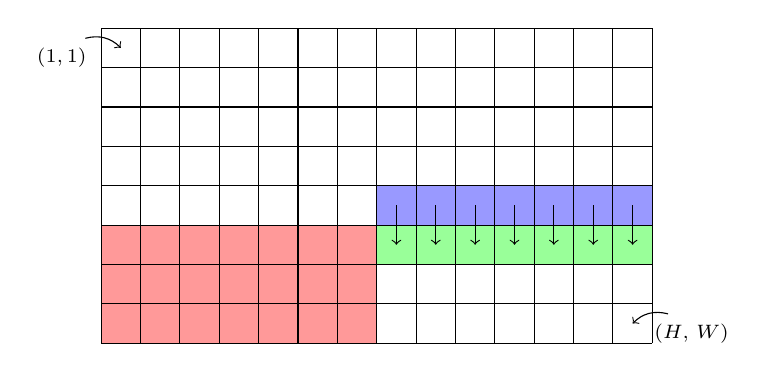
\begin{tikzpicture}[scale=0.5]

        \draw[fill=red!40] (0, 0) rectangle (7, 3);
        \draw[fill=blue!40] (7, 3) rectangle (14, 4);
        \draw[fill=green!40] (7, 2) rectangle (14, 3);

        \draw (0, 0) grid (14, 8);

        \node (A) at (-1, 7.25) { \scriptsize ($1, 1$) };
        \coordinate (B) at (0.5, 7.5);

        \node (X) at (15, 0.25) { \scriptsize ($H$, $W$) };
        \coordinate (Y) at (13.5, 0.5);

        \draw[->] (A) edge[bend left] (B);
        \draw[->] (X) edge[bend right] (Y);

        \draw[->] (7.5, 3.5) -- (7.5, 2.5);
        \draw[->] (8.5, 3.5) -- (8.5, 2.5);
        \draw[->] (9.5, 3.5) -- (9.5, 2.5);
        \draw[->] (10.5, 3.5) -- (10.5, 2.5);
        \draw[->] (11.5, 3.5) -- (11.5, 2.5);
        \draw[->] (12.5, 3.5) -- (12.5, 2.5);
        \draw[->] (13.5, 3.5) -- (13.5, 2.5);

    \end{tikzpicture}

\end{figure}
